\begin{landscape}
\begin{figure}[!ht]
\centering
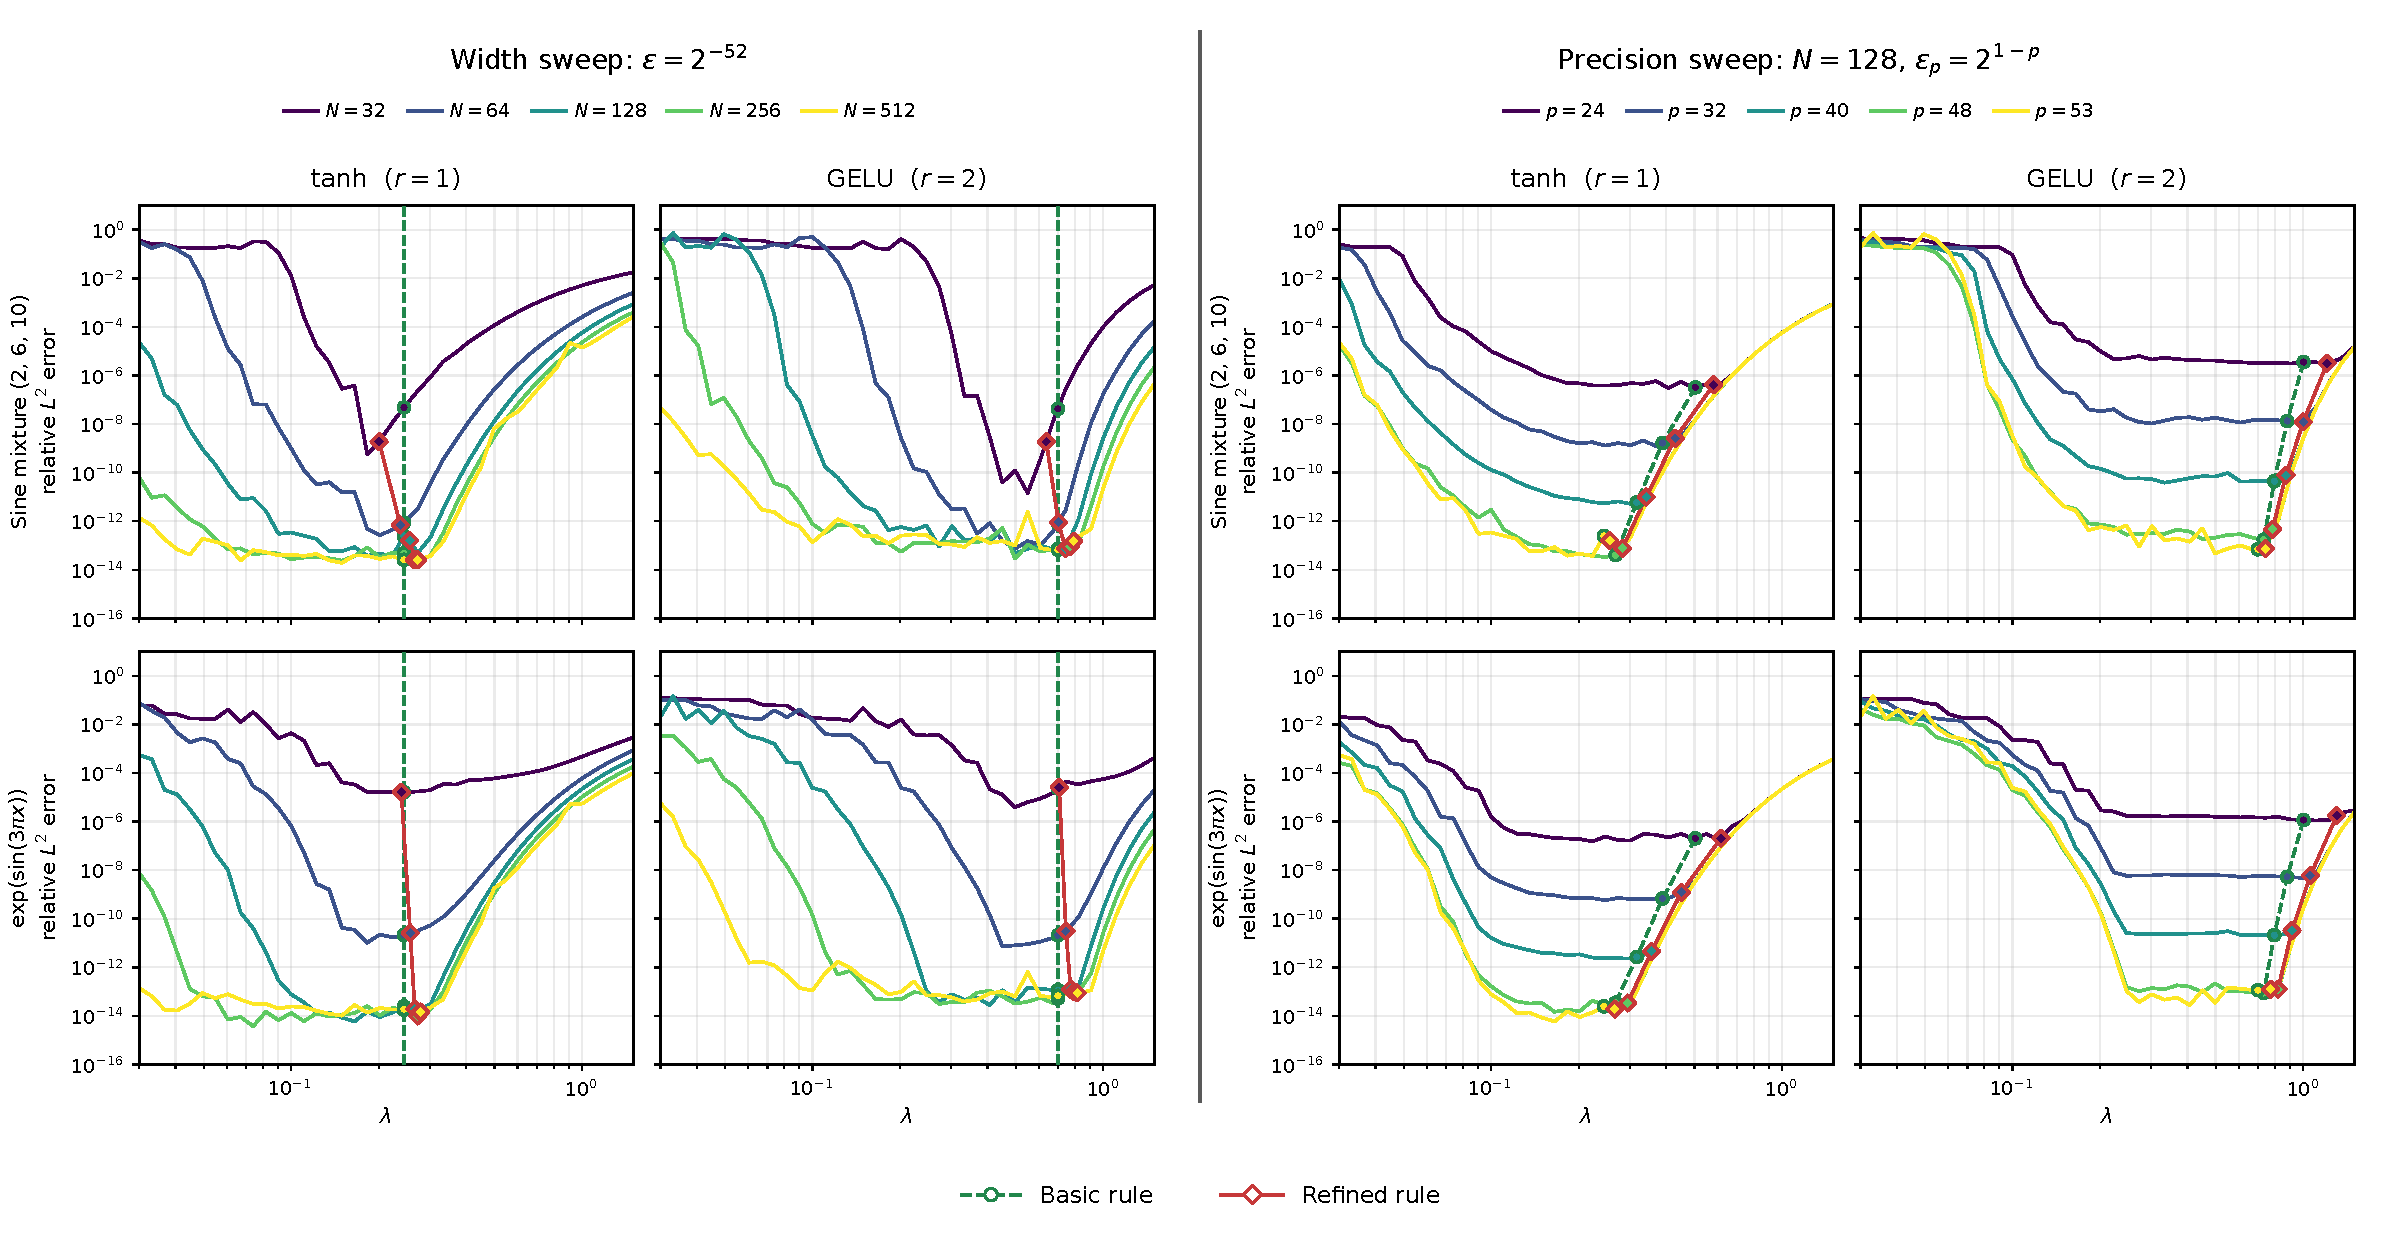
\includegraphics[width=\linewidth]{figures/lambda_rule_grid.pdf}
\caption{Basic (green, dashed) and refined (red, solid) bandwidth choices. The top row uses $\sin(2\pi x)+\tfrac12\sin(6\pi x)+\tfrac14\sin(10\pi x)$; the bottom uses $\exp(\sin(3\pi x))$. The left four panels vary $N\in\{32,64,128,256,512\}$ at $\varepsilon=2^{-52}$; the right four vary $p\in\{24,32,40,48,53\}$ at $N=128$, with effective tolerance $e_{\mathrm{tol}}=2^{1-p}$. At $p=16$, the refined GELU choices exceed the measured $\lambda$ range, so that precision is omitted from both activations. The refined choices solve the displayed first-pair equation using a rough frequency scale and no amplitude input. Curves use expC08's viridis colors, logarithmic axes, and original measured least-squares errors. Rule markers sit on the corresponding observed curves at the predicted bandwidths, so their vertical coordinates are measured, not predicted. Lines connect choices across settings; the width-independent basic choice is shown as a vertical line. Each network has $N+65$ activation neurons plus bias. Reduced precisions emulate rounding while solver internals remain fp64. The GELU panels use the general spectral score; the finite-contour theorem applies to tanh.}
\label{fig:lambda-grid}
\end{figure}
\end{landscape}
